\vspace{1.5pc}
\section[Domain dan Data Penelitian]{Domain dan Data Penelitian}
\begin{spacing}{1.5}
	\subsection[Domain Penelitian]{Domain Penelitian}
	Penelitian ini mengkaji hubungan antara IOD, parameter oseanografi (arus, temperatur, salinitas, MLD, Chl-a, fluks air tawar, fluks panas bersih) dan meteorologi (laju presipitasi dan tekanan angin) di Samudera Hindia dengan koordinat ($0^\circ-24.6^\circ$ N) dan ($78.2^\circ-105^\circ$ E) (lihat Gambar \ref{fig:domain}).

	\subsection[Data Penelitian]{Data Penelitian}
%	\vspace{-1pc}
%		\subsection[NEMO/CMEMS]{NEMO/CMEMS}
%	\par Model NEMO (\textit{Nucleus for European Modelling of the Ocean}) (\href{https://www.nemo-ocean.eu/}{https://www.nemo-ocean.eu/}) adalah model komputasi resolusi tinggi yang terus dikembangkan sejak tahun 2008 oleh konsorsium Eropa yang terdiri dari 5 institusi, yaitu CMCC, CNRS, \textit{Mercator Ocean}, \textit{Met Office}, dan NERC. Model ini digunakan untuk penelitian dan peramalan dalam bidang oseanografi dan klimatologi, dengan tujuan menjadi alat yang fleksibel untuk mempelajari fenomena fisik dan biogeokimia dalam sirkulasi laut, serta interaksinya dengan komponen sistem iklim Bumi, pada skala ruang dan waktu yang berbeda  \shortcite{madec_gurvan_2022_6334656}. Data \textit{output} model NEMO dapat diperoleh dari website CMEMS (\textit{Copernicus Marine Environment Monitoring Service}) \href{https://resources.marine.copernicus.eu/products}{(https://resources.marine.copernicus.eu/products)}. CMEMS merupakan w
%	
%	Data yang tersedia pada website CMEMS dapat dilihat pada Tabel . Resolusi data \textit{output} yang digunakan untuk model ini adalah dx = dy = 5 menit pada bidang horizontal dan 50-lapisan $(k \in [1,50])$ dengan ketebalan berbeda pada bidang vertikal:
%	\begin{equation*}
%		\begin{aligned}
%			z_k = \{0.49, 1.54, 2.65, 3.82, 5.08, 6.44, 7.93, 9.57, 11.40, 13.47, 15.82, 18.50, \\
%			21.60, 25.21, 29.44, 34.43, 40.34, 47.37, 55.76, 65.81, 77.85, 92.33, 109.73, 130.67, \\
%			155.85, 186.12, 222.47, 266.04, 318.13, 380.21, 453.94, 541.089, 643.57, 763.33, \\
%			902.34, 1062.44, 1245.29, 1452.25, 1684.28, 1941.89, 2225.08, 2533.33, 2865.70,  \\
%			3220.82, 3597.03, 3992.48, 4405.22, 4833.29, 5274.78, 5727.92 \} (m). \\
%		\end{aligned}
%	\end{equation*}
%	\subsection[HYCOM]{HYCOM}
%	\par Model HYCOM (\textit{HYbrid Coordinate Ocean Model}) (\href{https://www.hycom.org}{https://www.hycom.org}) adalah salah satu model sirkulasi laut (OGCM) yang menggunakan model numerik tiga dimensi Navier-Stokes dengan input data batimetri dari GEBCO (\textit{General Bathymetric Chart of the Oceans}), data asimilasi hidrografi laut dari NCODA (\textit{Navy Coupled Ocean Data Assimilation}) dan komponen meteorologi dari NCEP (\textit{National Centers for Environmental Prediction}) ataupun NAVGEM (\textit{The NAVy Global Environmental Model}) berupa tekanan angin, kecepatan, fluks panas, tekanan permukaan laut, presipitasi, temperatur, dan kelembapan \shortcite{JosephMetzger2013}. 
%	
%	Koordinat vertikal dalam HYCOM adalah isopiknal di lautan terbuka yang terstratifikasi dan memiliki transisi yang mulus dan dinamis serta bergantung terhadap waktu pada medan daerah pesisir yang dangkal dan pada tingkat tekanan tetap di lapisan campuran permukaan atau lautan yang tidak terstratifikasi \shortcite{chassignet2017,Park2013}. Data HYCOM yang digunakan adalah data analisis global arus dan temperatur tiga dimensi dengan resolusi spasial 5 menit untuk longitude dan 2.5 menit untuk latitude selama 12 bulan (Januari - Desember) tahun 2021 dan dengan ketebalan bervariasi pada bidang vertikal, yaitu 40-lapisan $(k \in [1,40])$:
%	\begin{equation*}
%		\begin{aligned}
%			z_k = \{0.0, 2.0, 4.0, 6.0, 8.0, 10.0, 12.0, 15.0, 20.0, 25.0, 30.0, 35.0, 40.0, 45.0, 50.0, \\
%			60.0, 70.0,	80.0, 90.0, 100.0, 125.0, 150.0, 200.0, 250.0, 300.0, 350.0, 400.0, 500.0, 600.0,\\
%			700.0, 800.0, 900.0, 1000.0, 1250.0, 1500.0, 2000.0, 2500.0, 3000.0, 4000.0, 5000.0\} (m). \\
%		\end{aligned}
%	\end{equation*}
%	\subsection[J-OFURO3]{J-OFURO3}
%	\subsection[NCEP/NCAR]{NCEP/NCAR}
	Intensitas IOD direpresentasikan oleh gradien anomali suhu permukaan laut (SST) antara Samudera Hindia ekuator bagian barat ($50^\circ E-70^\circ E$ dan $10^\circ S-10^\circ N$) dan Samudera Hindia ekuator bagian tenggara ($90^\circ E-110^\circ E$ dan $10^\circ S-0^\circ N$). Gradien ini dinamakan sebagai \textit{Dipole Mode Index} (DMI) \cite{Jiang2021,Dwivedi2012}. Beberapa data yang digunakan dalam penelitian ini adalah data arus laut, temperatur laut, salinitas, MLD, dan Chl-a. Data-data ini dapat diperoleh dari website penyedia data \textit{Copernicus Marine Environment Monitoring Service} (CMEMS) (\href{https://resources.marine.copernicus.eu/products}{https://resources.marine.copernicus.eu/products}) dan \textit{HYbrid Coordinate Ocean Model} (HYCOM) (\href{https://www.hycom.org}{https://www.hycom.org}). Data lainnya adalah fluks air tawar, fluks panas bersih, laju presipitasi, dan tekanan angin yang bersumber dari \textit{National Centers for Environmental Prediction and the National Center for Atmospheric Research reanalysis 1} (NCEP/NCAR) (\href{https://psl.noaa.gov/data/gridded/data.ncep.reanalysis.html}{https://psl.noaa.gov/data/gridded/data.ncep.reanalysis.html})  \cite{Kalnay1996} dan J-OFURO3 yang merupakan generasi ketiga dari \textit{Japanese ocean flux data set} (\href{https://www.j-ofuro.com/en/}{https://www.j-ofuro.com/en/}) yang menggunakan pengamatan penginderaan jarak jauh \cite{Tomita2019}. 
	
	Hasil yang sangat baik diperoleh dengan membandingkan data suhu 3D (dalam Kelvin) CMEMS dengan data pengamatan \textit{in situ} pada kedalaman 0 hingga 5 m di Samudera Hindia. Hal ini tercermin dari nilai \textit{Root Mean Square} (RMS), untuk perbandingan \textit{in situ thematic centre} (INS TAC), dengan nilai 0.65, dan untuk data \textit{in situ} CORIOLIS, dengan nilai 0.44. Perbandingan data salinitas 3D (dalam satuan salinitas praktis (psu)) dengan data pengamatan \textit{in situ} juga menunjukkan hasil yang sangat baik. Nilai RMS pada kedalaman 0 hingga 5 m untuk data global dan Samudera Hindia masing-masing adalah 0.65 dan 0.204 (Lellouche et al., 2019). Sama halnya dengan perbandingan model CMEMS dan konsentrasi \textit{float} Chl-a (\textit{Biogeochemical-Argo} (BGC-Argo), data pengukuran). Hal ini ditunjukkan oleh koefisien korelasi dan \textit{Root Mean Square Error} (RMSE) masing-masing sebesar 0,81 dan 0,59 (Lamouroux et al., 2019).   
	
	Data yang digunakan dapat dilihat secara lengkap dalam Tabel \ref*{tab:data}.
	\begin{table}[H]
		\centering
		\caption{Rangkuman data penelitian}
		\label{tab:data}
		\resizebox{\textwidth}{!}{%
		\begin{tabular}{|l|l|l|l|l|}
			\hline
			No & Data               & Periode   & Sumber      & Referensi \\ \hline
			1  & DMI                & 1994-2021 & NOAA/PSL    & \cite{Saji2003}      \\ \hline
			2  & Arus               & 1994-2021 & CMEMS/HYCOM & \cite{Lellouche2018,Chassignet2007}      \\ \hline
			3  & Temperatur laut    & 1994-2021 & CMEMS/HYCOM & \cite{Lellouche2018,Chassignet2007}      \\ \hline
			4  & Salinitas          & 1994-2021 & CMEMS/HYCOM & \cite{Lellouche2018,Chassignet2007}     \\ \hline
			5  & MLD                & 1994-2021 & CMEMS       & \cite{Lellouche2018}      \\ \hline
			6  & Chl-a              & 1994-2021 & CMEMS		  & \cite{Lellouche2018}      \\ \hline
			7  & Fluks air tawar    & 1994-2017 & J-OFURO3    & \cite{Tomita2019}      \\ \hline
			8  & Fluks panas bersih & 1994-2017 & J-OFURO3    & \cite{Tomita2019}     \\ \hline
			9  & Laju presipitasi   & 1994-2021 & NCEP/NCAR   & \cite{Kalnay1996}      \\ \hline
			10 & tekanan angin              & 1994-2021 & NCEP/NCAR   & \cite{Kalnay1996}      \\ \hline
		\end{tabular}%
	}
	\end{table}
	\subsection[Pengumpulan Data]{Pengumpulan Data}
	Data dalam Tabel \ref{tab:data} merupakan data yang tersedia secara gratis dan bersifat terbuka. Data ini dapat diunduh secara langsung pada website penyedia data ataupun menggunakan kode skrip. Kode skrip yang digunakan untuk mengunduh data dengan bahasa \textit{Shell script} (terminal Linux) dan Python disajikan dalam Lampiran 1.
	
	\begin{figure}[H]
		\centering
		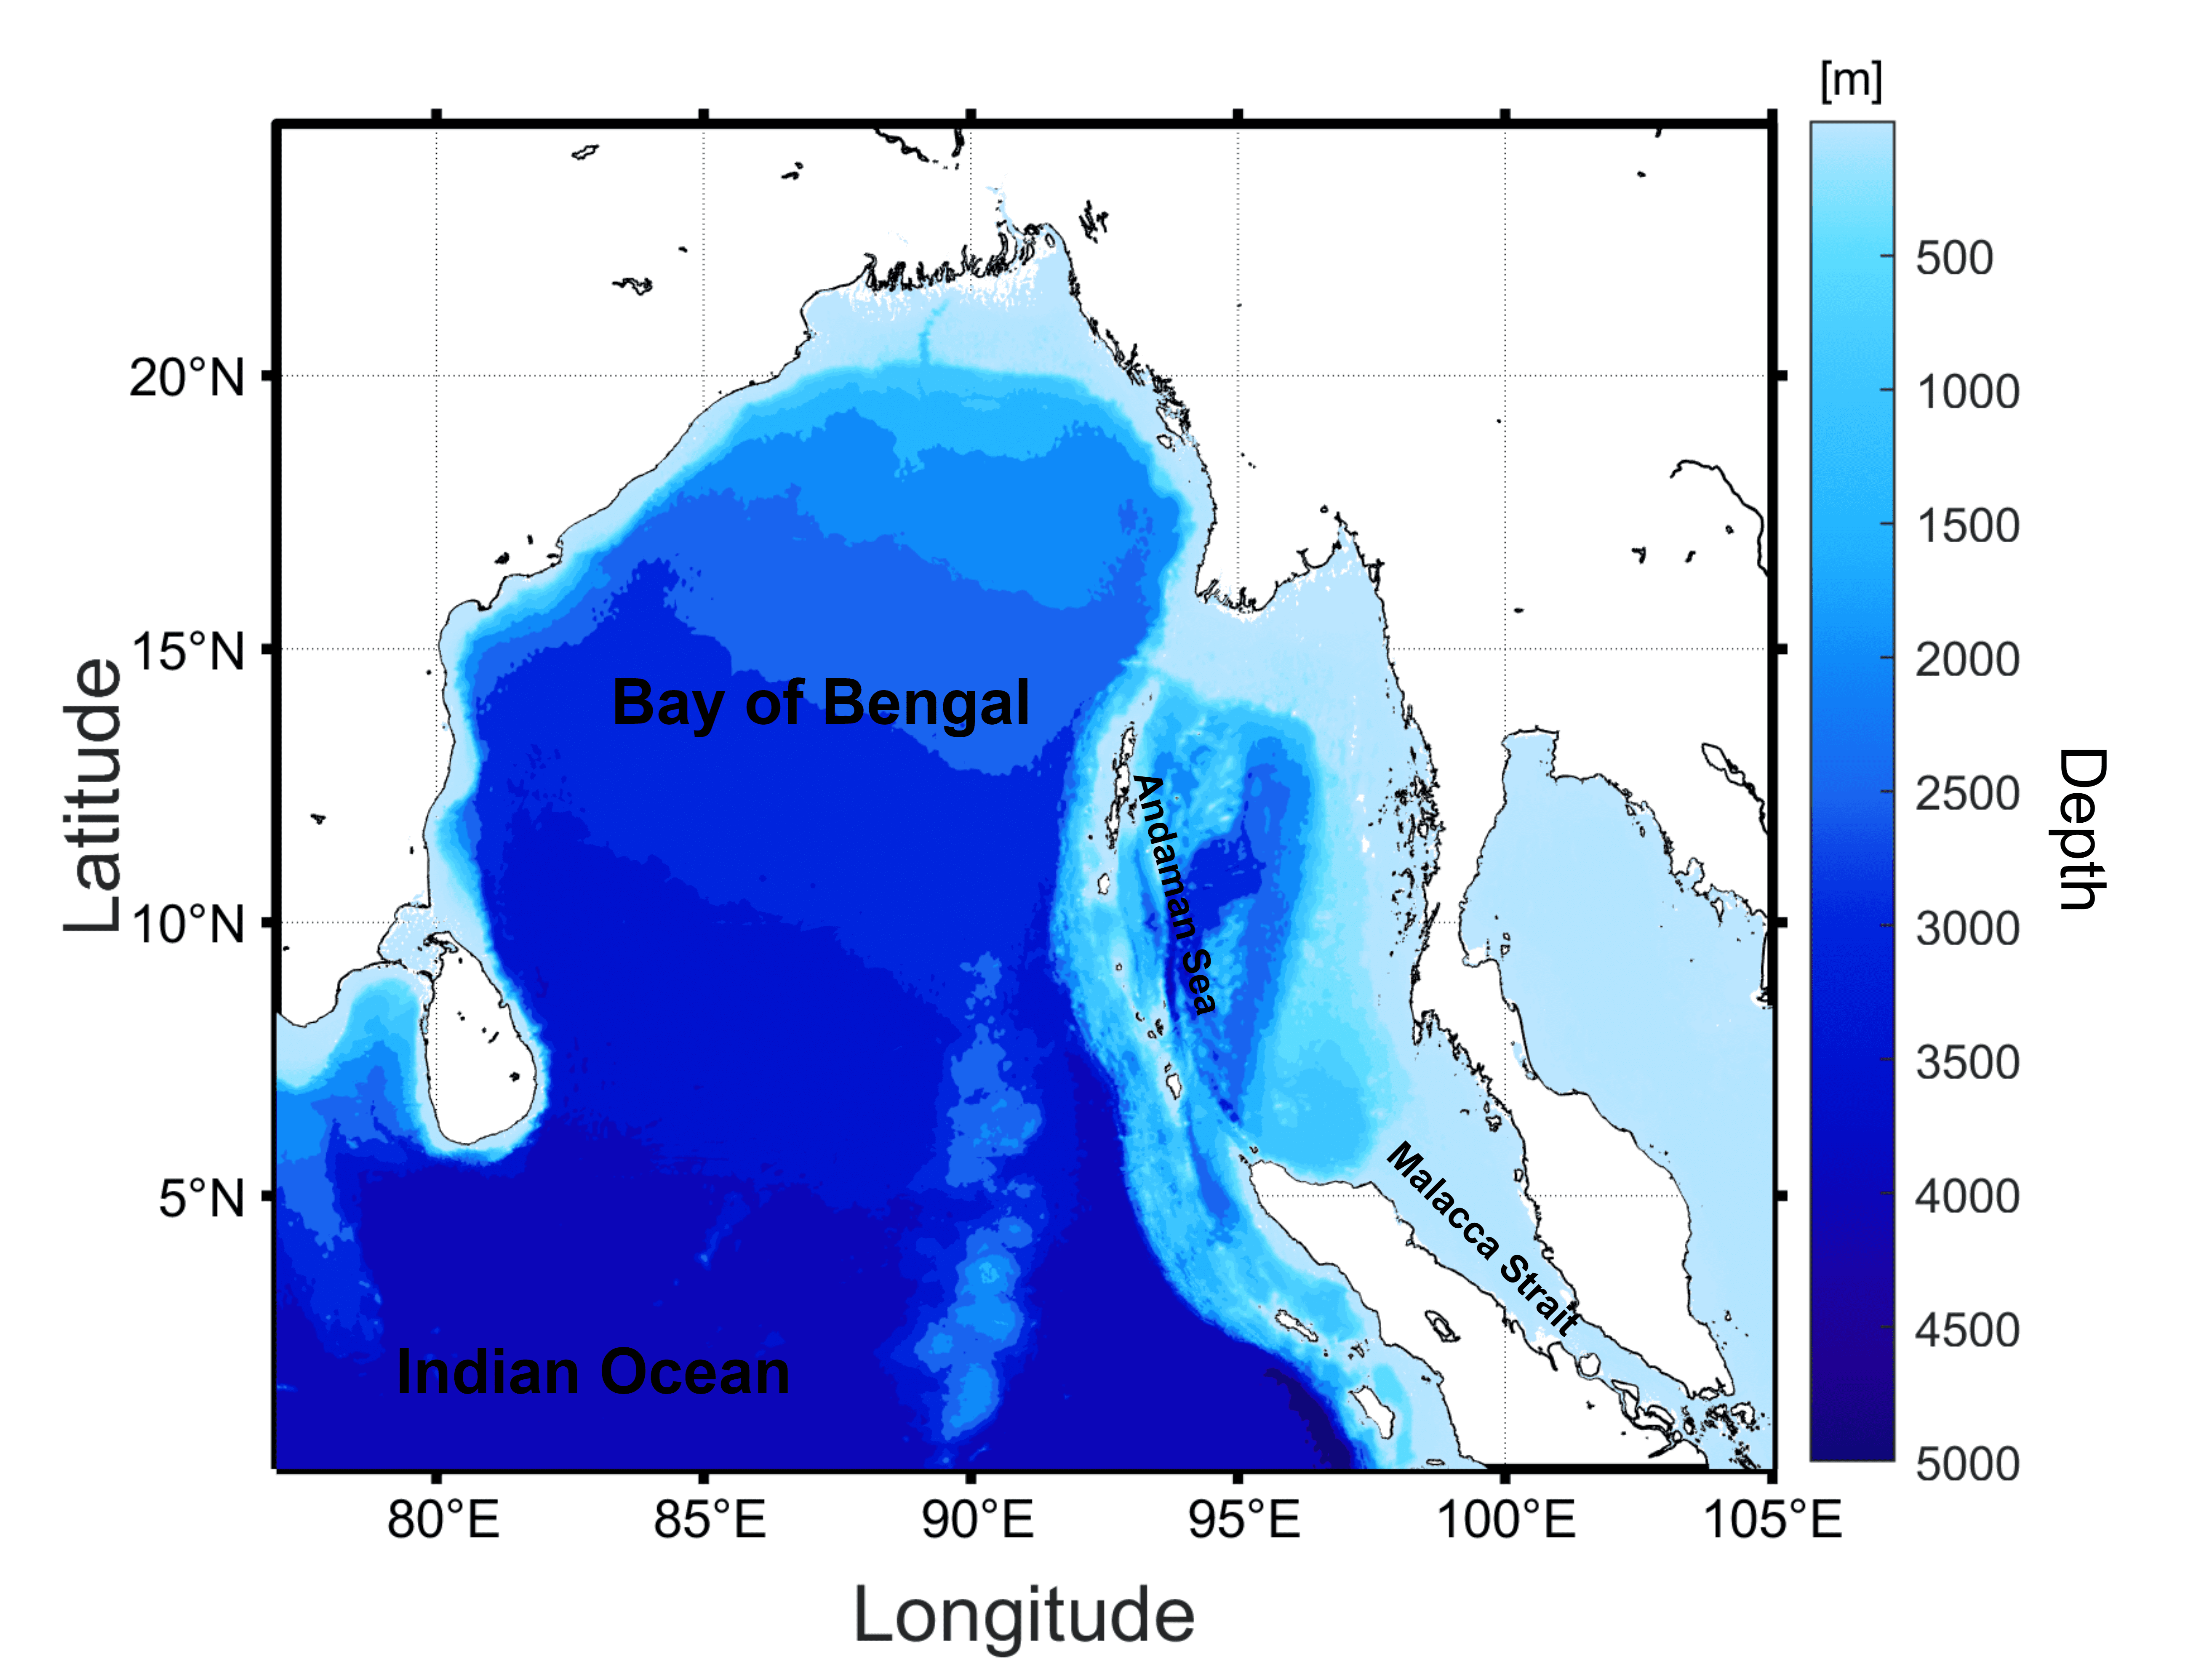
\includegraphics[width=12cm]{contents/Figures/Batimetri_edit_compress}
		\caption{Peta batimetri Samudera Hindia, diperoleh dari SRTM30+ \protect\cite{becker2009global}. Warna dalam peta menunjukkan kedalaman 0-5000 m sedangkan pulau digambarkan tanpa warna.}
		\label{fig:domain}
	\end{figure}
\end{spacing}
\vspace{-0.5pc}
\section[Analisis Data]{Analisis Data}
\begin{spacing}{1.5}
	\subsection[Model Musiman]{Model Musiman}
	Data jangka panjang dapat dianalisis dengan menggunakan analisis deret waktu, seperti contohnya adalah analisis model musiman, yang bertujuan untuk menganalisis kemungkinan adanya pola musiman yang berulang dalam periode tertentu pada data tersebut. Monsoon merupakan penyebab utama perubahan IOD, parameter oseanografi seperti arus, temperatur, salinitas, MLD, Chl-a, fluks air tawar, dan fluks panas bersih, serta parameter meteorologi seperti laju presipitasi dan angin. Penelitian ini akan menganalisis parameter-parameter tersebut dengan menggunakan model musiman yang didasarkan pada pola kejadian monsun. Model musiman ini digunakan untuk mengamati pola periodik dan memprediksi parameter-parameter berdasarkan keteraturan mereka. Dengan cara ini, akan diketahui apakah parameter yang diteliti mengikuti pola monsun yang terjadi, apakah terjadi pergeseran bulanan pada masing-masing parameter dalam model musiman yang dibangun, serta apakah parameter-parameter tersebut mengikuti pola monsun yang sama.
	
	Beberapa penelitian yang menggunakan model musiman adalah \shortciteauthor{Haridhi2016} \citeyear{Haridhi2016} yang meneliti tentang hubungan antara \textit{sea surface temperatur} (SST) dan \textit{net deployment} (ND) - penyebaran jaring nelayan pukat cincin tradisional. \shortciteauthor{Ikhwan2022} \citeyear{Ikhwan2022} dalam penelitiannya mengkaji tentang kedalaman lapisan campuran (MLD) di laut Andaman menggunakan data \textit{sea surface salinity} (SSS) dari model 3-D \textit{Copernicus Marine Environment Monitoring Service} (CMEMS). \shortciteauthor{hidayat2023relationship} \citeyear{hidayat2023relationship}, mengkaji tentang hubungan antara SST, SSS, dan Chl-a di \textit{Northern Bay of Bengal} (NBoB). 
	
	Persamaan siklus musiman \cite{crawley2012r} dapat dituliskan sebagai
	\begin{equation}\label{eq:sm_}
		y = \alpha + \beta \sin(2\pi t)+\gamma \cos(2\pi t) + \epsilon,
	\end{equation}
	dengan $\alpha, \beta$, dan $\gamma$  adalah konstanta pergesaran vertikal, amplitudo dari gelombang sinus, dan amplitudo dari gelombang kosinus. Dalam persamaan ini, $t$ adalah waktu dan $\epsilon$ adalah elemen residual yang mewakili komponen \textit{white-noise} tidak beraturan dalam proses pengambilan data. 
	
	Gambar \ref{fig:sm} merupakan ilustrasi persamaan \ref{eq:sm_} untuk nilai $\alpha,\beta$ dan $\gamma$ yang berbeda. Nilai $\alpha$ yang berbeda mempengaruhi posisi kurva terhadap sumbu-y. Sedangkan nilai $\beta$ dan $\gamma$ yang berbeda mempengaruhi posisi kurva terhadap sumbu-x.
	\begin{figure}[H]
		\centering
		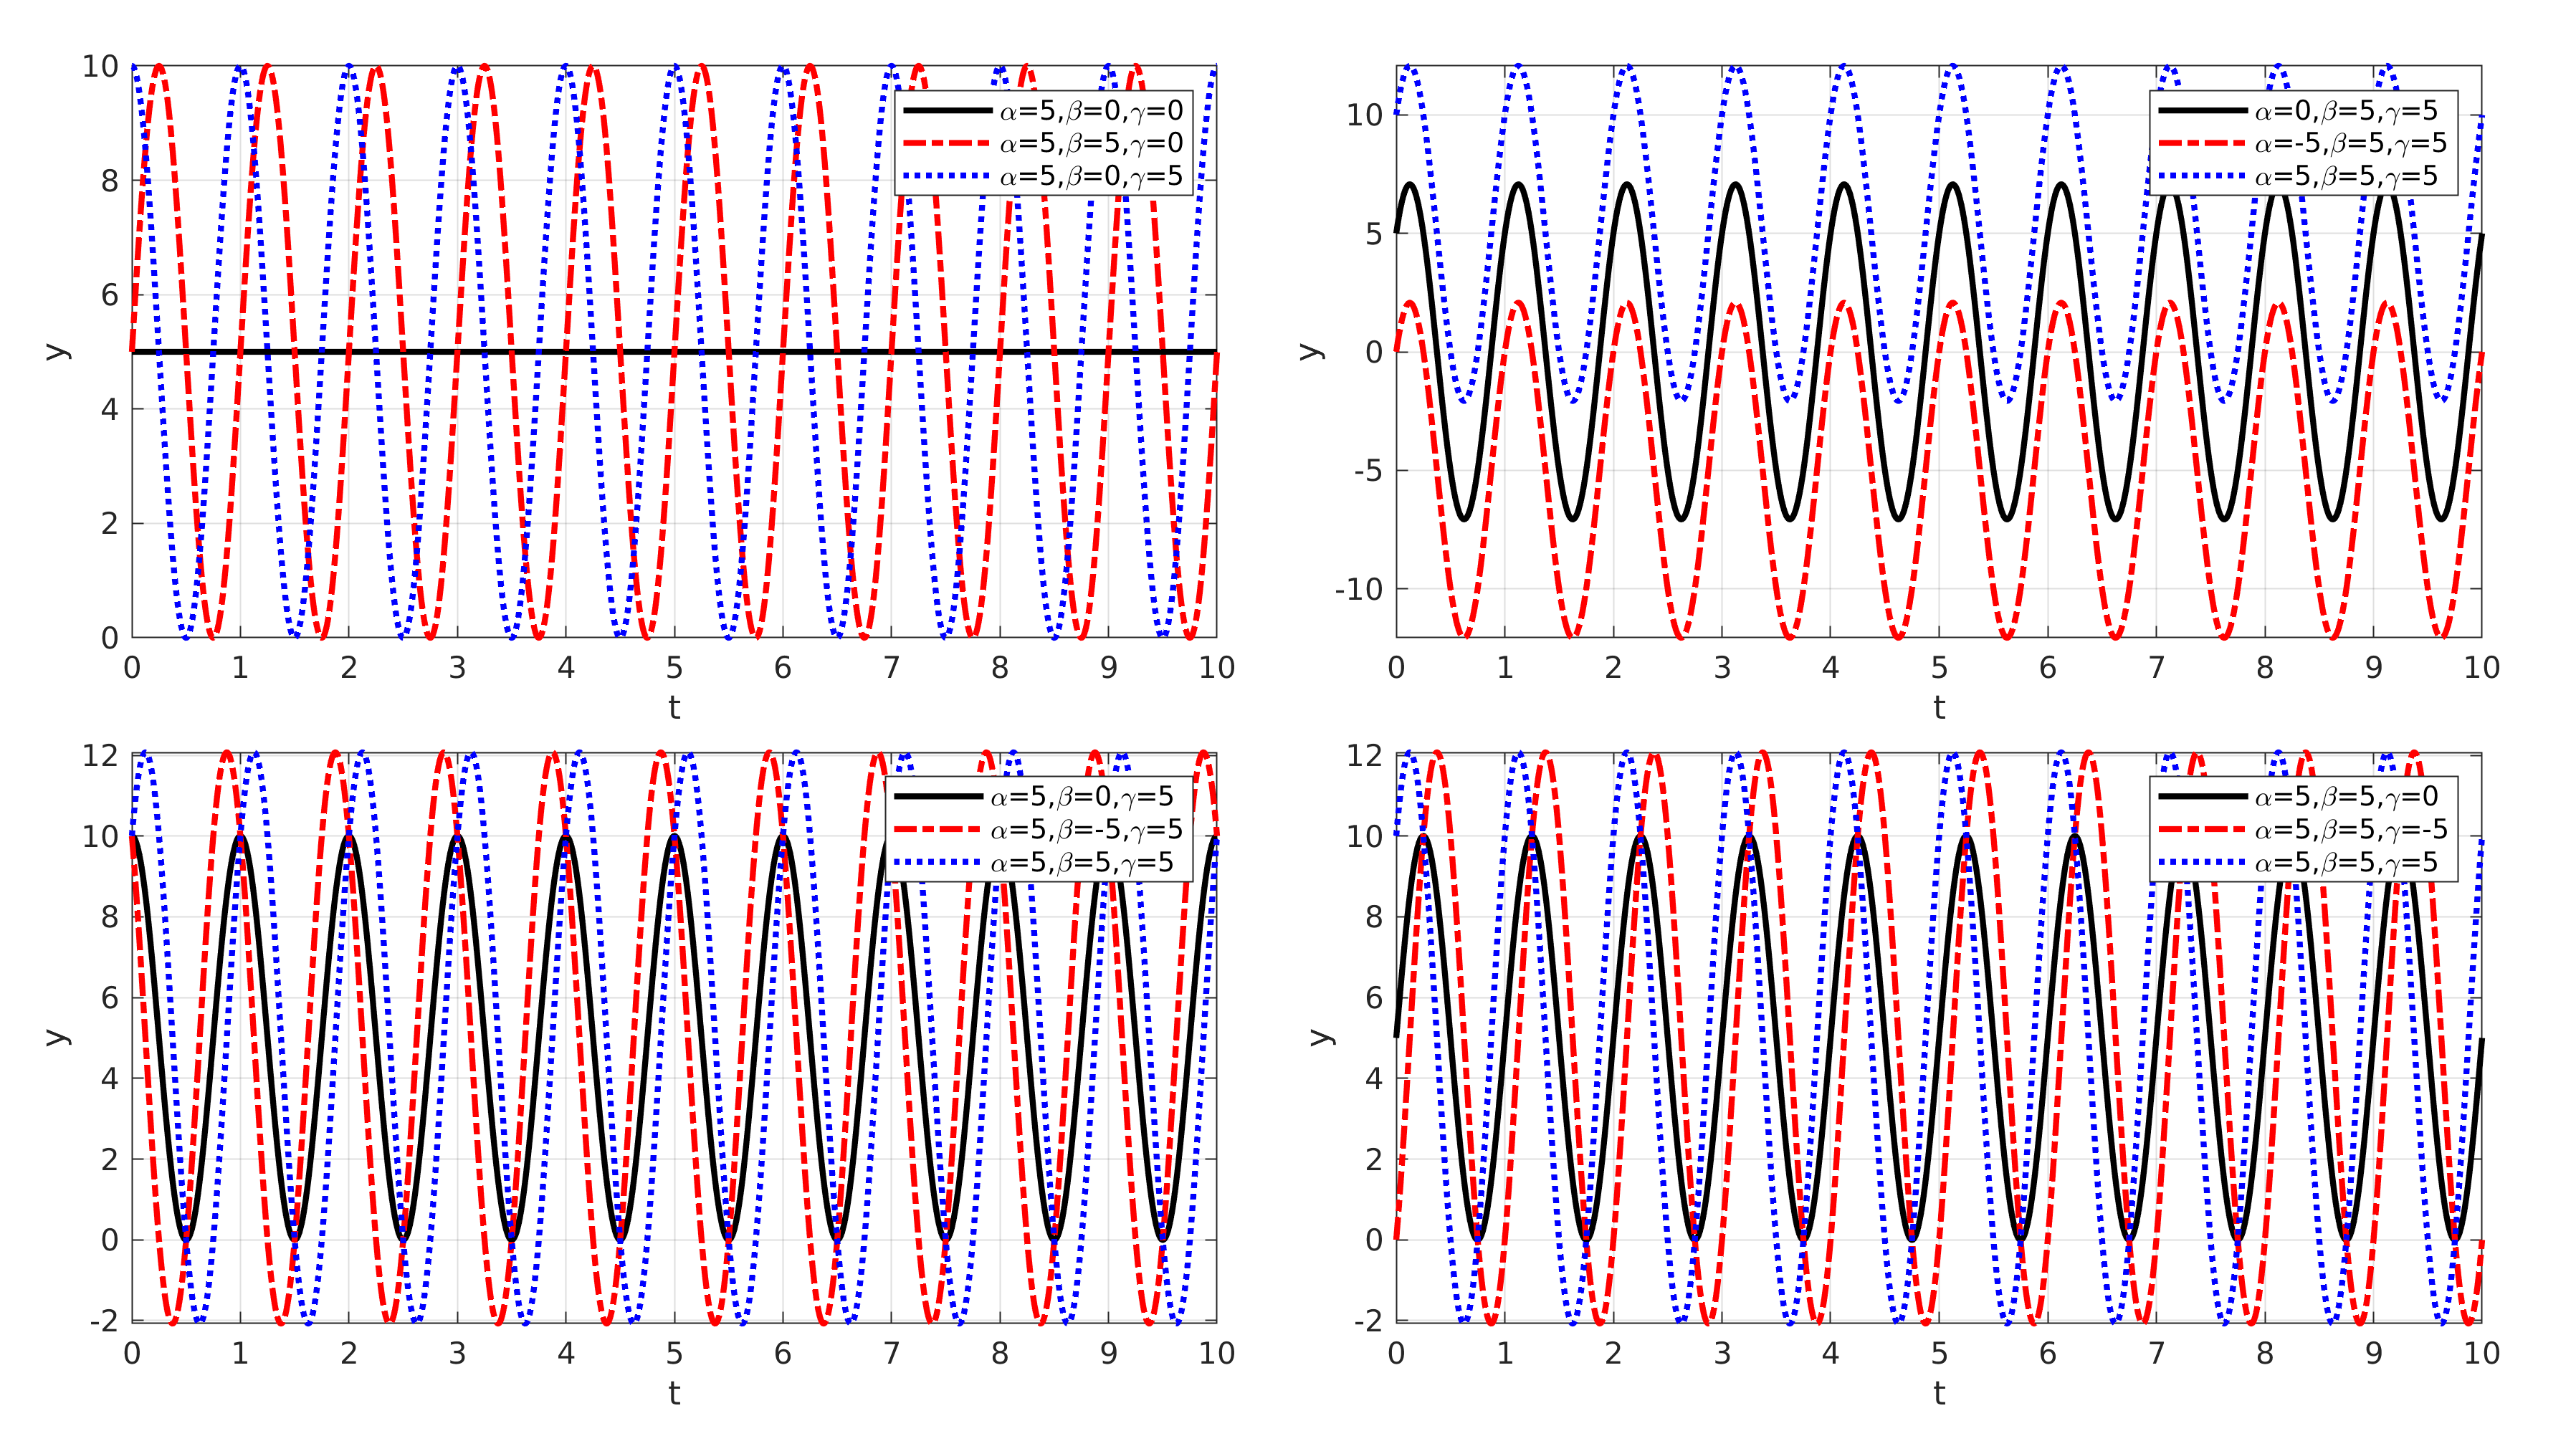
\includegraphics[width=15cm]{contents/Figures/sm_experiment}
		\caption{Ilustrasi persamaan model musiman.}
		\label{fig:sm}
	\end{figure}
	
%	Langkah-langkah yang digunakan untuk menggambarkan \textit{seasonal model} dapat dijelaskan sebagai berikut.
%	\begin{itemize}
%		\item \textbf{\textit{Start}}. \textit{Software} yang digunakan untuk menentukan nilai $\alpha, \beta$ dan $\gamma$ adalah \textit{software} \textit{R}.
%		\item \textbf{\textit{Initialization}}. Dalam proses inisialisasi ini, komponen musiman semua parameter dimodelkan untuk mendapatkan siklus tahunan.
%		\item \textbf{\textit{Input}}. Setelah proses inisialisasi \textit{input} parameter yang ingin diprediksi kemudian dimasukkan.
%		\item \textbf{\textit{Process}}. Selanjutnya dilakukan perhitungan dengan menggunakan fungsi model linear (\verb|lm()|) dalam \textit{R}.
%		\item \textbf{\textit{Output}}. Perintah Summary() digunakan untuk menampilkan hasil dalam proses sebelumnya. Dalam tahapan ini juga diperoleh penggambaran \textit{seasonal model}.
%	\end{itemize}

	\subsection[Analisis Korelasi]{Analisis Korelasi}
		 Analisis korelasi berfungsi sebagai alat eksplorasi data dan pembuatan hipotesis terkait hubungan antara parameter yang diteliti. Dalam penelitian ini, analisis korelasi digunakan untuk mengukur kekuatan (nilai koefisien korelasi) dan arah (positif/negatif) hubungan antara indeks IOD dengan parameter lainnya, serta untuk menentukan signifikansi koefisien korelasi tersebut.
		
		Penelitian ini menganalisis hubungan antara IOD, parameter oseanografi (arus, temperatur, salinitas, MLD, Chl-a, fluks air tawar, fluks panas bersih) dan meteorologi (laju presipitasi dan tekanan angin). Persamaan korelasi dan koefisien korelasi yang digunakan dapat dituliskan sebagai \cite{hidayat2023relationship,Haditiar2020}
		\begin{equation}
			\begin{aligned}
				y &= a+rx\\
				r &= \frac{\sum (x_i - \bar{x})(y_i - \bar{y})}{\sqrt{\sum (x_i-\bar{x})^2\sum (y_i-\bar{y})^2}},
			\end{aligned}
		\end{equation}
		dengan $\alpha$ adalah konstanta titik potong sumbu-$y$, $r$ adalah kemiringan dari garis regresi (koefisien regresi), $x_i, y_i$ adalah variable yang digunakan untuk menghitung koefisien korelasi dengan $i$ adalah indeks data. Sedangkan $\bar{x}$ dan $\bar{y}$ adalah rata-rata. 
%		Persamaan untuk t-statistik dapat dituliskan sebagai
%		\begin{equation}
%			\begin{aligned}
%				t=\frac{r_{xy}\sqrt{n-2}}{1-r^2_{xy}}.
%			\end{aligned}
%		\end{equation}
%		Jika $\|t\|\geq t_{\text{tabel}}$ dengan ($\alpha=5\%$) maka terdapat korelasi antara $x$ dan $y$.
\end{spacing}
\vspace{-0.5pc}
\section[Prosedur Penelitian]{Prosedur Penelitian}
\begin{spacing}{1.5}
	Prosedur penelitian mengikuti diagram alir pada Gambar \ref{fig:flowchart} dan dapat dijelaskan sebagai berikut. 
	\begin{itemize}
		\item \textbf{\textit{Start}}. \textit{Software} yang digunakan dalam penelitian ini adalah Matlab dan \textit{R}.
		\item \textbf{\textit{Input}}. Data-data terkait penelitian yang akan digunakan sebagai \textit{input} diunduh terlebih dahulu.
		\item \textbf{\textit{Process}}. Setelah data tersedia, kemudian data diolah dengan cara melakukan pemetaan dan penggambaran data.
		\item \textbf{\textit{Output}}. Hasilnya adalah peta IOD, oseanografi, dan meteorologi secara jangka panjang. 
		\item \textbf{\textit{Process}}. Tahapan selanjutnya adalah analisis data. Dalam tahap ini dilakukan analisis model musiman (\textit{seasonal model}) untuk mengidentifikasi pola musiman dan memprediksi parameter berdasarkan keteraturannya. Dilakukan juga analisis statistik, dalam hal ini analisis korelasi untuk melihat hubungan IOD, parameter oseanografi dan meteorologi.
		\item \textbf{\textit{Output}}. Terakhir, diperoleh kesimpulan berdasarkan analisis yang telah dilakukan.
		\item \textbf{\textit{End}}. Penelitian selesai.
	\end{itemize}
	\begin{figure}[H]
		\centering
		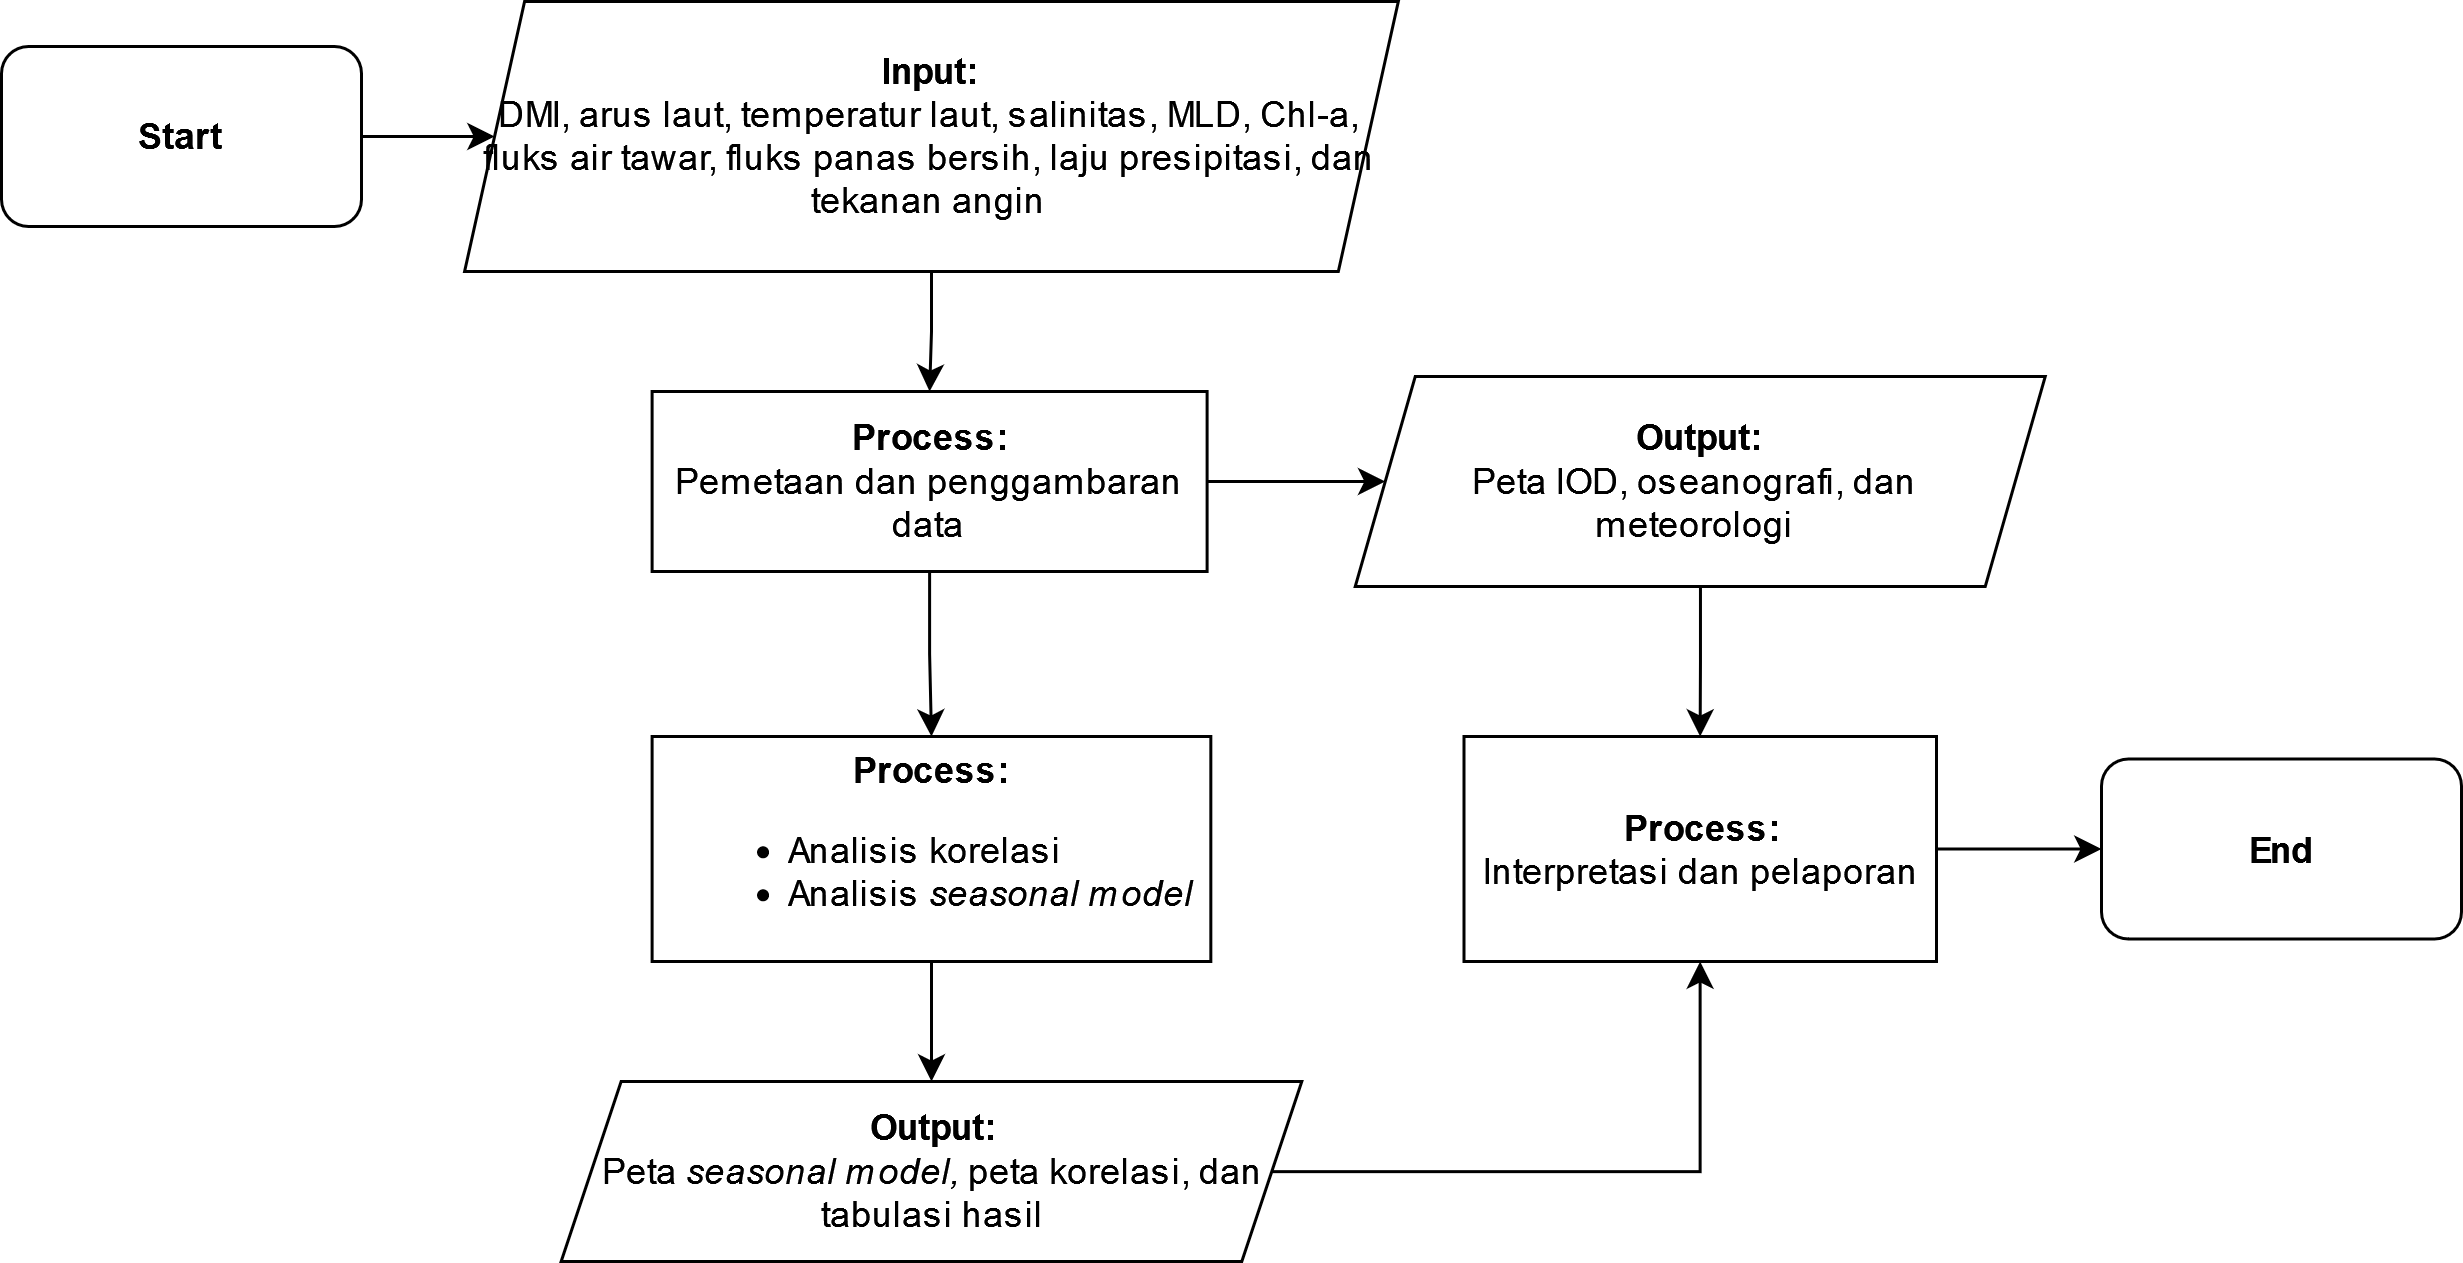
\includegraphics[width=10cm]{contents/Figures/Flowchart_Diagram.png}
		\caption{Diagram alir penelitian}
		\label{fig:flowchart}
	\end{figure}
\end{spacing}
